\documentclass[manuscript,review,anonymous]{acmart}
\setcopyright{none}
\settopmatter{printacmref=false}
\acmDOI{}
\acmISBN{}
\acmConference[CHI 2027 submission]{CHI 2027 Posters submission}{}{}
\acmYear{2027}
\title{The Delegation Blind Spot: Auditing Product Decisions from Agent Choices}
\begin{document}
\begin{abstract}
An agent's successful choice need not tell a product team which future improvement its customer would value. We present a decision-specific audit that reports compatible product-value intervals and the population mixtures attaining their endpoints. In 4,800 API requests across two pinned models and one synthetic task family, the conservative audit resolves none of 36 comparisons, despite different execution accuracy. An exploratory follow-up records supplied preferences instead of actions: it resolves three of nine comparisons per model at matched observation counts. This is extraction of known input, not discovery of human preferences. We introduce a source-labeled decision receipt and an offline diagnostic viewer, and distinguish structural ambiguity from finite-sample uncertainty through controlled channels. The contribution is a reproducible measurement workflow and interface-design question, not a new general inference method or human validation.
\end{abstract}
\ccsdesc[500]{Human-centered computing~Human computer interaction (HCI)}
\ccsdesc[300]{Computing methodologies~Artificial intelligence}
\keywords{AI delegates, decision support, measurement design, partial identification, agent telemetry}
\maketitle

\section{The analyst's decision differs from the agent's task}
Two agents book the same hotel, one for quiet and the other for proximity to a meeting. Both bookings can be optimal, yet the transaction alone cannot distinguish demand for soundproofing from demand for transport links. The analyst asks about a future change. Human choices can share this ambiguity; delegation does not create a new impossibility theorem.

We ask: \emph{does a declared log support a declared product comparison under an explicit calibration model?} Our executable audit exposes compatible decisions and assumptions, using actual model responses to synthetic objectives, controlled channels, and an evidence interface. It does not estimate actual demand.

Work on delegated choice, preference transmission, and revealed-preference alignment already studies how agent behavior relates to principals' preferences \cite{kops2026,kraft2026,suleymanov2026}. Rich variation across menus can identify quantities that coarse transaction categories cannot. Controlled agent-choice experiments also have direct precedents \cite{cherep2025}. Our operational focus is a particular future product contrast and the uncertainty left by a specified logging scheme. The statistical foundations are established experiment comparison, label-shift estimation, and measurement-error partial identification \cite{blackwell1953,lipton2018,finkelstein2021}.

\begin{figure}[t]
\centering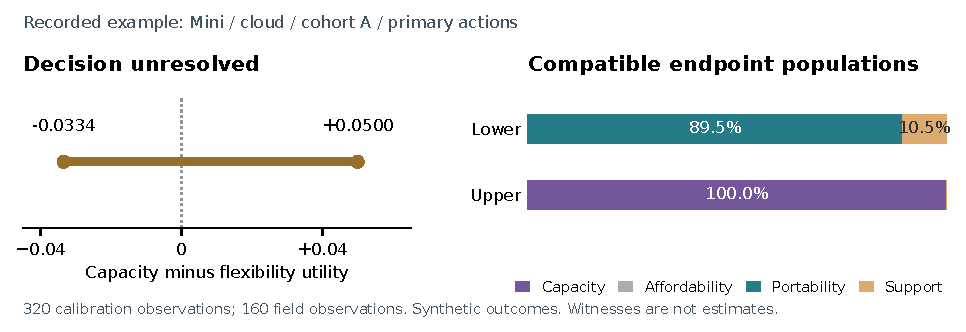
\includegraphics[width=\linewidth]{../generated/audit-example.pdf}
\caption{A compact rendering of one recorded inspector condition. Opposite endpoints are attained by different mixtures within the same uncertainty restrictions; they need not share one exact channel. Both remain compatible with the observed counts.}
\Description{The recorded contrast interval runs from minus 0.0334 to plus 0.0500 and crosses zero. Its lower witness is approximately 89.5 percent portability-first and 10.5 percent support-first; the upper witness is 100 percent capacity-first. These are compatible synthetic populations, not estimates of real people.}
\label{fig:audit}
\end{figure}

\section{A calibrated decision audit}
Let $p$ contain the proportions of $K$ declared intent classes. A column-stochastic channel $A$ maps class to logged category, so $q=Ap$. Each class has a separately specified value difference $d_k$ between product variants. The target and its compatible range are
\begin{equation}
\Delta=d^Tp,\qquad [L,U]=\left[\min_{p\geq0,\,\mathbf1^Tp=1,\,Ap=q}d^Tp,\ \max_{p\geq0,\,\mathbf1^Tp=1,\,Ap=q}d^Tp\right].
\end{equation}
A positive lower endpoint supports variant one throughout this model; a negative upper endpoint supports variant zero. Otherwise the audit abstains and reports endpoint witness mixtures. The witnesses are compatible populations, not reconstructed individuals.

For known $A$, a standard linear identification fact is that $d^Tp$ is identified from $q$ for every feasible log distribution $q$ precisely when $d$ lies in the row space of $A$. If $d=A^Tv$, the contrast equals $v^Tq$; otherwise a null-space direction changes the contrast without changing the observations. This structural question differs from whether a finite sample supplies a narrow interval.

We propagate calibration and field-frequency uncertainty through a joint-mass linear program. With $J_{ak}=A_{ak}p_k$, impose $p\geq0$, $\mathbf1^Tp=1$, $\sum_aJ_{ak}=p_k$, $J\geq0$, $\underline A_{ak}p_k\leq J_{ak}\leq\overline A_{ak}p_k$, and $\underline q_a\leq\sum_kJ_{ak}\leq\overline q_a$. Optimizing $d^Tp$ gives attainable bounds within these rectangular restrictions. Simultaneous coordinate Clopper--Pearson bounds allocate errors $.02$ to calibration and $.02$ to the field, yielding at least 96\% \emph{marginal} coverage per predeclared comparison under independent sampling, stable channels, correct classes, and known $d$. This is neither simultaneous coverage across all reported comparisons nor protection against an incorrect outcome model. Infeasible programs return a diagnostic failure.

\section{Computational evaluation}
\paragraph{Design.}
The primary design was committed before API execution. GPT-5.4 Mini and Nano, pinned to their 17 March 2026 snapshots, each received the same 2,400 tasks. Three framings, travel, cloud plans, and workflow software, share one generator. Four synthetic profiles specify numerical attribute weights and a minimum-attribute penalty. Each menu contains four perturbed alternatives in randomized order. Per model and framing, calibration has 80 tasks per class; three field mixtures have 160 tasks each. Calibration labels are known from the constructed profiles. The field estimator does not receive them.

The future comparison is capacity versus flexibility investment with the same affordability tradeoff. Class contrasts are exact means of best attainable utility over an independent 4,096-menu bank. They assume optimal future selection, not future behavior measured from the tested model. This known synthetic contrast isolates the measurement problem; a real deployment would need independent outcome evidence. Logs retain either selected product type or type plus context, including failure categories. Both omit the full continuous menu.

\paragraph{Primary result.}
Of 4,800 attempts, 4,783 return valid choices and 17 have retained transport failures, without replacement retries. Mini chooses a utility maximizer in 73.19\% of field tasks; Nano does so in 55.69\%. Nevertheless, all 18 comparisons per model remain unresolved, including every comparison for the optimal-choice control. This does not demonstrate structural information loss. The observed fraction containing the synthetic target is not an empirical coverage estimate because conditions share data.

\paragraph{An explicit-information control.}
After inspecting the primary result, we froze a follow-up asking for the largest weight already supplied to the agent. It selects 40 calibration tasks per class and 80 field tasks per mixture and framing by task ID, independently of response correctness. Each model makes 1,200 new calls, but these repeat only 12 distinct prompts. A leading attribute uniquely identifies its constructed class. Every report is correct; a deterministic parser could supply the same field without an LLM. Table~\ref{tab:result} compares the resulting channel with original actions from the same task IDs. Only the positive mixture resolves in each framing. Observation counts are matched, not token cost, privacy exposure, or human elicitation burden. Reused field draws and the data-motivated follow-up receive no selective-inference correction, so these are exploratory descriptions.

\begin{table}[t]
\centering
\caption{Recorded results per model. Primary rows use 160 field tasks per condition; paired rows use 80. Intervals concern known synthetic utility differences. The parser uses a known identity channel; model reports retain estimated-channel uncertainty.}
\label{tab:result}
\begin{tabular}{lrrr}
\toprule Observation & Mini resolved & Nano resolved & Mean interval width \\\midrule
Primary action/context logs & 0/18 & 0/18 & n/a \\
Paired action-only logs & 0/9 & 0/9 & 0.08720 \\
Paired supplied-preference reports & 3/9 & 3/9 & 0.04360 \\
Deterministic supplied-weight parser & \multicolumn{2}{c}{7/9 (shared tasks)} & 0.02285 \\\bottomrule
\end{tabular}
\end{table}

\paragraph{Separating uncertainty sources.}
A controlled sensitivity analysis uses $A_\eta=(1-\eta)\mathbf1\mathbf1^T/4+\eta I_4$. At $\eta=0$, every class has the same action law. At every $\eta>0$, the channel is full rank: exact identification holds even when sampling intervals remain wide. Across six channel strengths, four calibration budgets, and three mixtures, 200 independent repetitions per cell produce 14,400 multinomial datasets. With $\eta=.01$, 2,560 calibration observations per class and 5,120 field observations still leave all joint intervals unresolved, despite exact identification. Known-channel, known-frequency, and jointly uncertain ablations isolate the sources of imprecision. Their marginal guarantees are 98\%, 98\%, and 96\%, respectively; they are not an equal-confidence ranking. Settings and Monte Carlo intervals accompany the artifact.

\paragraph{Preserving structured input directly.}
A deterministic parser removes model-report calibration uncertainty: on the same 720 field records it resolves 7/9 comparisons using a known identity channel and 96\% marginal field intervals, with zero incorrect resolutions and no calibration or API calls. Direct Hoeffding intervals for the bounded class contrast also resolve 7/9, reported separately rather than intersected. These controls distinguish structural ambiguity, sampling precision, and avoidable report-channel calibration uncertainty; they are not new model responses or human observations.

\section{A decision receipt for an analyst}
The offline viewer exposes intervals and witness mixtures by model, framing, mixture, and log schema (Fig.~\ref{fig:audit}), alongside contrast definitions and observation counts. It renders recorded LP outputs without recomputation or LLM queries. Usability and decision impact remain unmeasured.

A proposed \emph{decision receipt} separates the source of each claim. For example, a hotel record may contain an \textbf{observed} booking, a \textbf{supplied} quiet-room constraint, an \textbf{inferred} preference for boutique hotels, and a \textbf{confirmed outcome} marked missing. An inferred explanation must not acquire the status of customer evidence merely because an agent states it confidently. The receipt links these fields to a future decision, agent/interface version, and assigned probe. The experiment tests one supplied field, not the entire proposed interface.

Three design implications follow. Preserve relevant structured input before paying an agent to reconstruct it. Preserve the measurement condition, since pooling probe identities can erase information. Treat an unresolved decision as a request to diagnose the information gap, not automatically to collect more of the same log. Direct, consented outcome measurement may be preferable to inferring latent intent. Key open questions concern which fields merit retention, how consent and burden constrain that choice, and whether analysts interpret witness populations correctly.

\section{Scope, provenance, and artifacts}
This computational work uses one synthetic task family and two related model snapshots. It establishes neither human preference validity nor a general relationship between agent capability and analyst information. Unknown classes, drift, dependent provider failures, and an incorrect product contrast can invalidate the model. A receipt identifying a supplied profile does not validate that profile against its user. There are no human participants or measured customer outcomes.

\paragraph{AI-assisted research methods.}
OpenAI Codex assisted with problem formulation, literature retrieval, proof drafting, experiment design, implementation, analysis, figures, and manuscript preparation. Internal AI critiques were used during revision and are not independent peer review. Checks include primary-source comparison, mathematical counterexamples, numerical witness verification, unit tests, immutable response records, and exact reanalysis. These checks do not replace human-author scrutiny and accountability. The models under test and their experimental roles are distinct from this research-assistance workflow.

\paragraph{Availability.}
The research artifacts include code, proofs, frozen designs, response provenance, controls, and the offline viewer. Identifying links are omitted for anonymous review. Commercial effectiveness remains untested.

\bibliographystyle{ACM-Reference-Format}
\bibliography{../references}
\end{document}
